\subsection{Frontend}
\label{subsec:kelvin-frontend}

Frontendová část systému je z technologického hlediska výrazně komplikovanější než backend, protože v době psaní práce prochází historickým vývojem, který zanechal vrstvení tří různých technologií v jednom projektu.

Nejstarší vrstvou jsou Django šablony (\textit{Django templates}) -- serverově generované HTML stránky, které byly původním způsobem tvorby uživatelského rozhraní.
Django šablony jsou stále přítomny v systému u statičtějších částí rozhraní, kde není potřeba dynamického chování na straně klienta.

Druhou vrstvou je \textit{Svelte} -- moderní JavaScript framework pro tvorbu reaktivních komponent na straně klienta.
V průběhu vývoje systému Kelvin byl Svelte adoptován jako primární framework pro dynamické části rozhraní, zejména pro zobrazení a přidávání komentářů ke zdrojovému kódu.
Svelte komponenty jsou v produkci kompilovány do čistého JavaScriptu bez runtime knihovny, což zajišťuje rychlé načítání.
Tato vrstva je však již považována za zastaralou a nové funkcionality v ní aktuální už nejsou vyvíjené.

Třetí a v současnosti preferovanou vrstvou je \textit{Vue.js} -- JavaScript framework, na který systém aktivně migruje.
Vue.js bylo zvoleno jako nástupce Svelte zejména z důvodu větší komunity, lepší dlouhodobé podpory a nižší vstupní bariéry pro nové přispívatele.

Výsledkem tohoto historického vývoje je stav, kdy se ve zdrojovém kódu systému souběžně nacházejí všechny tři frontendové technologie.
Dopady tohoto stavu na vývoj nových funkcionalit jsou rozvedeny v \secref[sekci]{sec:kelvin-development} a celková architektura systému je znázorněna na \figref{fig:kelvin-architecture}.

\begin{figure}[H]
    \centering
    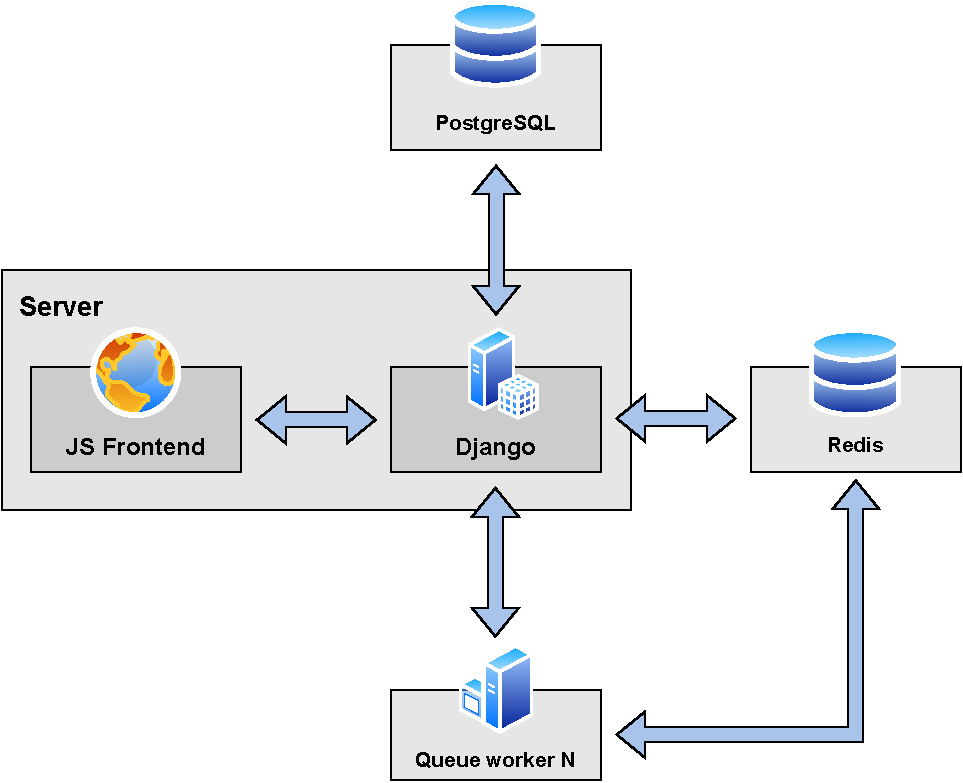
\includegraphics[width=0.85\textwidth]{resources/diagrams/kelvin-architecture}
    \caption{Zjednodušená architektura systému Kelvin}{Zjednodušená architektura systému Kelvin~\cite{kelvin-architecture}}
    \label{fig:kelvin-architecture}
\end{figure}

\endinput
